\chapter{Επίλογος}
Στο τελευταίο κεφάλαιο, πραγματοποιείται συνοπτική παρουσίαση των θεμάτων που αναλύθηκαν έως τώρα. Στη συνέχεια παρουσιάζονται τα συμπεράσματα που προέκυψαν κατά τη διαδικασία σχεδίασης και κατασκευής της διαδικτυακής εφαρμογής.
Επιπλέον, γίνεται λεπτομερής ανάλυση SWOT (Strengths, Weaknesses, Opportunities, Threats) του συστήματος, καθώς και προτάσεις για μελλοντικές βελτιστοποιήσεις και επεκτάσεις των λειτουργιών που παρέχει.

\section{Ανακεφαλαίωση Διπλωματικής Εργασίας}
Οι ανάγκες δικτυακής εκκίνησης υπολογιστών του Εργαστηρίου Ρομποτικής, Ενσωματωμένων και Ολοκληρωμένων Συστημάτων του Πανεπιστημίου Δυτικής Μακεδονίας, απαιτούσαν μια διαδικτυακή εφαρμογή με συγκεκριμένα χαρακτηριστικά και δυνατότητες που δεν ήταν διαθέσιμες σε εμπορικές λύσεις. Για την κάλυψη αυτών των αναγκών, αναπτύχθηκε η διαδικτυακή εφαρμογή `iBoot'.

Η εφαρμογή `iBoot' αναπτύχθηκε χρησιμοποιώντας PHP στο back-end και HTML, CSS, JavaScript και Bootstrap στο front-end. Τα δεδομένα της εφαρμογής αποθηκεύονται σε μια σχεσιακή βάση δεδομένων MySQL. Η πρόσβαση στην εφαρμογή μπορεί να γίνει είτε μέσω μιας διεπαφής χρήστη είτε μέσω ενός REST API που αναπτύχθηκε για αυτόν το σκοπό. Ο πηγαίος κώδικας της εφαρμογής είναι διαθέσιμος στο κοινό και έχει δημοσιευτεί υπό τους όρους της άδειας MIT.

Η εφαρμογή διευκολύνει την πρόσβαση σε τρεις τύπους χρηστών.

Ένας ανώνυμος χρήστης έχει πρόσβαση μόνο στις σελίδες σύνδεσης, εγγραφής και υπενθύμισης των διαπιστευτηρίων σύνδεσης.
Ο διαχειριστής εργαστηρίου μπορεί να διαχειρίζεται υπολογιστές σε συγκεκριμένα εργαστήρια. Μπορούν επίσης να τοποθετηθούν υπολογιστές σε εργαστήρια που διαχειρίζεται ο διαχειριστής και οι οποίοι δεν έχουν ήδη τοποθετηθεί σε άλλα εργαστήρια.
Ο διαχειριστής μπορεί να χρησιμοποιεί όλες τις δυνατότητες της πλατφόρμας χωρίς περιορισμούς. Ο διαχειριστής έχει την εξουσία να προσθέτει, να αφαιρεί και να τροποποιεί υπολογιστές, ομάδες, εργαστήρια, μπλοκ iPXE, μενού εκκίνησης, χρονοδιαγράμματα και χρήστες. Ο Διαχειριστής επιτρέπεται επίσης να βλέπει τα αρχεία καταγραφής συμβάντων της εφαρμογής.
Εν κατακλείδι,
Οι υπολογιστές επικοινωνούν με συγκεκριμένες σελίδες της εφαρμογής για να εγγραφούν και να λάβουν μενού εκκίνησης.

Η εφαρμογή έχει σχεδιαστεί και υλοποιηθεί σύμφωνα με τις βέλτιστες πρακτικές και τα πιο πρόσφατα πρότυπα ασφαλείας για την προστασία των πληροφοριών που περιέχονται σε αυτήν. Οι κωδικοί πρόσβασης των χρηστών αποθηκεύονται στη βάση δεδομένων της εφαρμογής αφού υποστούν επεξεργασία μέσω κρυπτογραφικά ασφαλών συναρτήσεων κατακερματισμού και δεν εμφανίζονται ποτέ στην εφαρμογή. Η πιστοποίηση ταυτότητας και τα δικαιώματα του χρήστη που επιθυμεί να προβάλει τη σελίδα ελέγχονται πριν από τη φόρτωση, ενώ το API υλοποιεί την ίδια διαδικασία προσθέτοντας σε κάθε αίτηση JWT tokens. Η εφαρμογή είναι σε θέση να λειτουργεί τόσο με το πρωτόκολλο HTTP όσο και με το πιο ασφαλές πρωτόκολλο HTTPS και μπορεί ακόμη και να κρυπτογραφήσει τα cookies συνόδου.

Το Εργαστήριο Ρομποτικής, Ενσωματωμένων και Ολοκληρωμένων Συστημάτων του Πανεπιστημίου Δυτικής Μακεδονίας θα εκσυγχρονίσει τη διαδικασία διαχείρισης του μενού εκκίνησης του δικτύου των υπολογιστών του με την εγκατάσταση της διαδικτυακής εφαρμογής "iBoot", η οποία θα διευκολύνει επίσης σημαντικά την καταγραφή και την παρακολούθηση των υπολογιστών αυτών.

\section{Μοντέλο Ανάλυσης S.W.O.T.}

\subsection{Τι είναι το Μοντέλο Ανάλυσης S.W.O.T.;}


\subsection{Ανάλυσης S.W.O.T. της εφαρμογής iBoot}
Στο σχήμα \ref{fig:iBoot_swot_analysis} απεικονίζεται η ανάλυση S.W.O.T. της εφαρμογής iBoot. Τα ευρήματα της ανάλυσης αναλύονται στη συνέχεια, το καθένα στην αντίστοιχη υποενότητα.

\begin{figure}[ht]
	\centering
	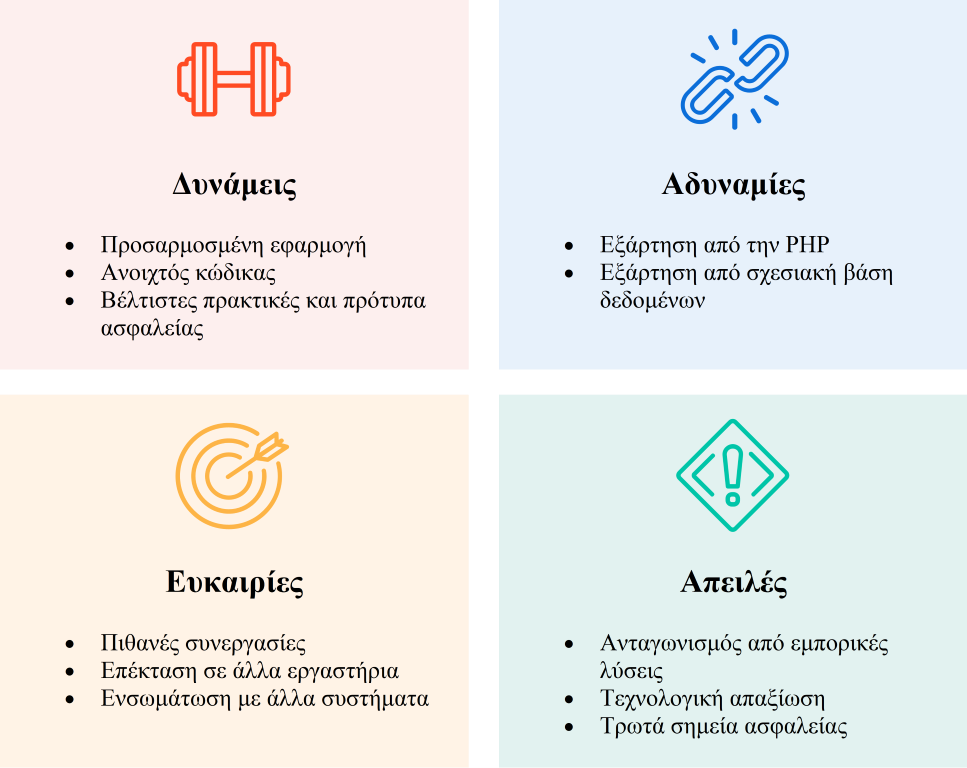
\includegraphics[scale=0.5]{swot-analysis.png}
	\caption{Ανάλυση SWOT εφαρμογής iBoot}
	\label{fig:iBoot_swot_analysis}
\end{figure}

\subsubsection{Δυνάμεις}
\begin{description}
	\item[Προσαρμοσμένη εφαρμογή:] Η εφαρμογή iBoot αναπτύχθηκε ειδικά για να ανταποκρίνεται στις απαιτήσεις του Εργαστηρίου Ρομποτικής, Ενσωματωμένων και Ολοκληρωμένων Συστημάτων, διασφαλίζοντας ότι διαθέτει τα απαραίτητα χαρακτηριστικά και δυνατότητες.
	\item[Ανοιχτός κώδικας:] Ο πηγαίος κώδικας της εφαρμογής είναι διαθέσιμος στο κοινό και δημοσιεύεται με την άδεια MIT, επιτρέποντας τη διαφάνεια και τις πιθανές συνεισφορές της κοινότητας.
	\item[Βέλτιστες πρακτικές και πρότυπα ασφαλείας:] Η εφαρμογή έχει σχεδιαστεί και υλοποιηθεί σύμφωνα με τις βέλτιστες πρακτικές και τα πιο πρόσφατα πρότυπα ασφαλείας, διασφαλίζοντας την προστασία των πληροφοριών και την κρυπτογράφηση των cookies συνόδου.
\end{description}

\subsubsection{Αδυναμίες}
\begin{description}
	\item[Εξάρτηση από την PHP:] Το back-end της εφαρμογής iBoot είναι κατασκευασμένο με τη χρήση PHP, η οποία μπορεί να δημιουργήσει προκλήσεις όσον αφορά την επεκτασιμότητα και τη συμβατότητα με μελλοντικές τεχνολογίες.
	\item[Εξάρτηση από σχεσιακή βάση δεδομένων:] Η εφαρμογή βασίζεται σε μια σχεσιακή βάση δεδομένων MySQL για την αποθήκευση δεδομένων, γεγονός που ενδέχεται να περιορίσει την επεκτασιμότητα και την απόδοση κατά τον χειρισμό μεγάλων όγκων δεδομένων.
\end{description}

\subsubsection{Ευκαιρίες}
\begin{description}
	\item[Πιθανές συνεργασίες:] Η φύση της εφαρμογής ως ανοικτού κώδικα δημιουργεί ευκαιρίες συνεργασίας με άλλα ιδρύματα ή προγραμματιστές που μπορούν να συμβάλουν στην περαιτέρω βελτίωσή της.
	\item[Επέκταση σε άλλα εργαστήρια:] Η επιτυχία και ο θετικός αντίκτυπος της εφαρμογής iBoot στο Εργαστήριο Ρομποτικής, Ενσωματωμένων και Ολοκληρωμένων Συστημάτων μπορεί να οδηγήσει στην υιοθέτησή της από άλλα εργαστήρια εντός του Πανεπιστημίου Δυτικής Μακεδονίας ή και πέραν αυτού.
	\item[Ενσωμάτωση με άλλα συστήματα:] Η εφαρμογή μπορεί να διερευνήσει ευκαιρίες για ενσωμάτωση με άλλα συστήματα ή πλατφόρμες, επιτρέποντας βελτιωμένη λειτουργικότητα και διαλειτουργικότητα.
\end{description}

\subsubsection{Απειλές}
\begin{description}
	\item[Ανταγωνισμός από εμπορικές λύσεις:] Παρόλο που η εφαρμογή iBoot αναπτύχθηκε για να ικανοποιήσει συγκεκριμένες απαιτήσεις, υπάρχει πιθανότητα ανταγωνισμού από εμπορικές λύσεις που μπορεί να προσφέρουν περισσότερα χαρακτηριστικά ή ευρύτερο φάσμα δυνατοτήτων.
	\item[Τεχνολογική απαξίωση:] Οι ταχείες εξελίξεις στην τεχνολογία ενδέχεται να καταστήσουν ορισμένες πτυχές της εφαρμογής ξεπερασμένες, απαιτώντας συνεχείς ενημερώσεις και προσαρμογές για να παραμείνει επίκαιρη.
	\item[Τρωτά σημεία ασφαλείας:] Παρά την τήρηση των βέλτιστων πρακτικών και των προτύπων ασφαλείας της εφαρμογής, υπάρχει ο κίνδυνος τρωτών σημείων ασφαλείας και πιθανών παραβιάσεων, οι οποίες θα μπορούσαν να θέσουν σε κίνδυνο τις πληροφορίες και τη λειτουργικότητα της εφαρμογής.
\end{description}

\section{Μελλοντικές Επεκτάσεις}

Περαιτέρω ανάπτυξη του REST API.
Αναπτυξη αλλου front-end αξιοποιωντας το REST API.

\section{Συμπεράσματα}

\section{Σύνοψη Κεφαλαίου 6}
Το κεφάλαιο 6 σηματοδοτεί το πέρας της παρούσας διπλωματικής εργασίας. Στο παρόν κεφάλαιο παρέχεται μια ανάλυση SWOT του περιεχομένου της διαδικτυακής πλατφόρμας, η οποία περιγράφει συνοπτικά τα πλεονεκτήματα και τα μειονεκτήματα που σχετίζονται με την υλοποίηση του παρόντος έργου, καθώς και τις δυνατότητες και τα οφέλη που παρουσιάζει και τυχόν πιθανούς κινδύνους που μπορεί να αντιμετωπίσει. Παρέχονται επίσης ορισμένες ιδέες για πιθανές μελλοντικές βελτιώσεις και προσαρμογές της πλατφόρμας. Το κεφάλαιο αυτό ολοκληρώνεται με τα τελικά συμπεράσματα επί της διπλωματικής εργασίας.
